\chapter{Méthodologie}
\section{Introduction}
Au cours des chapitres précédents, nous avons exploré les différents types d'algorithmes et d'apprentissage automatique et d'apprentissage profond, ainsi que la notion de classification. En se basant sur ces concepts,
ce chapitre se concentre sur l'expérimentation de la construction de modèles de réseaux de neurones artificiels dans deux scénarios : avec compression de données en utilisant l’algorithme des components principales (ACP) et sans compression de données. Nous appliquerons également différents types d'algorithmes d'optimisation. Les résultats les tests et les évaluations seront enregistrés afin de déterminer l'efficacité des techniques utilisées et de comparer les modèles construits.

\section{Notre  Objectif}
Cette étude vise à mettre en évidence l'importance de l'utilisation des données basé
 sur un étude statistique préalable dans la construction des modèles 
 de prédiction supervisée. Nous menons une analyse comparative pour évaluer 
 l'impact de la compression des données sur les algorithmes de classification profonde, ainsi que l'étendue de l'impact des algorithmes d'optimisation. Pour ce faire, nous avons utilisé un ensemble de données sur lesquels nous avons réalisé ces tests.

 \begin{figure}[!p]
    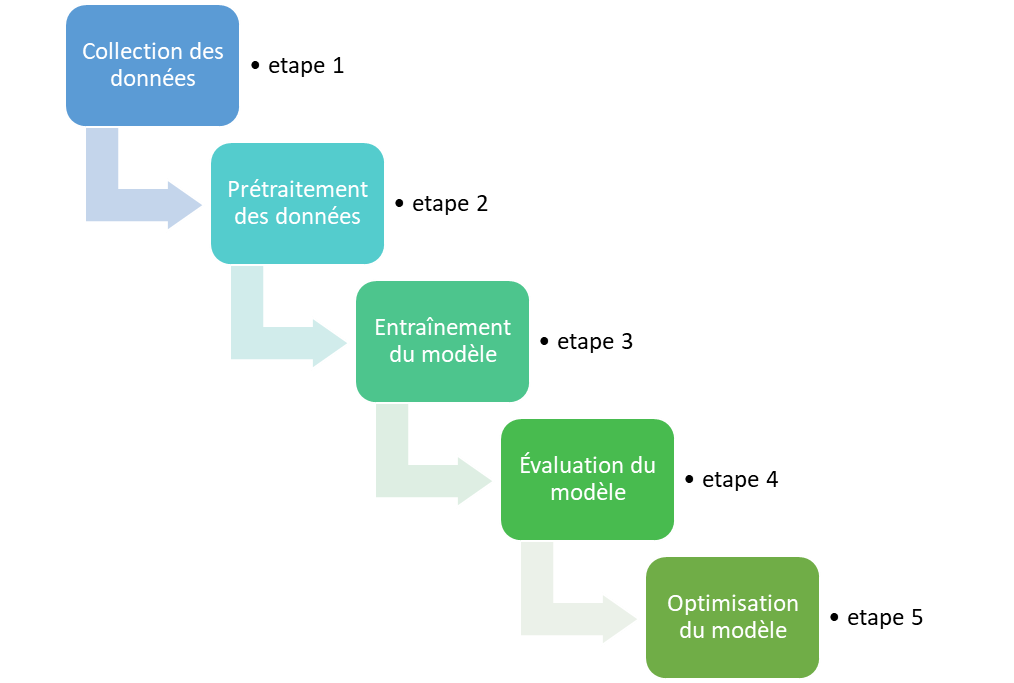
\includegraphics[scale=0.5]{Images/Chapter4/etapes.png}
    \caption{Tux, le pingouin}
    \label{fig:18}
    \end{figure}
\section{Prétraitement}
Le prétraitement des données, également connu sous le nom de nettoyage des données, représente une phase cruciale dans l'analyse de données. Cette étape englobe la transformation des données brutes en données exploitables en éliminant les erreurs, les valeurs manquantes, les doublons, et en les standardisant dans un format approprié. Les étapes suivantes illustrent le processus de prétraitement des données que nous avons effectué :
/\begin{enumerate}
    \item \textbf{Collection des Données}: Pour cette étude,  nous avons  exploré et choisi un jeu de données approprié sur la plateforme \textbf{Kaggle}, comprenant environ 5 000 enregistrements en tenant compte de sa pertinence par rapport aux objectifs spécifiques de  notre cas d'étude. Après avoir récupéré le jeu de données, nous avons effectué des ajustements pour l'adapter aux exigences et aux paramètres définis dans le cadre de notre étude.
    \item \textbf{Importation des Données}: Pour l'importation de données dans l'environnement \textbf{Python}, il est courant de recourir à la bibliothèque \textbf{Pandas}, renommée pour sa capacité à gérer divers formats de fichiers de données. Plus précisément, la fonction \textbf{read\_csv()} de pandas est souvent utilisée pour importer des données à partir de fichiers au format \textbf{CSV.} Cette fonctionnalité permet de charger les données contenues dans un fichier CSV dans une structure de données appelée \textbf{DataFrame }, offrant ainsi une manipulation et une analyse aisées des données dans Python.
    \item \textbf{Répartition des Données Entraînement et Test}: Dans notre étude, nous avons effectué une étape cruciale de division des données de l’ensemble d'entraînement et de test. Nous avons attribué 80\% des données à l'ensemble d'entraînement, tandis que les 20\% restants ont été réservés à l'ensemble de test. Cette répartition nous a permis de disposer d'un ensemble suffisamment large pour entraîner nos modèles tout en conservant un ensemble distinct pour évaluer leur performance. Cela garantit une évaluation fiable de la capacité de généralisation de nos modèles sur des données qu'elles n'ont pas encore vues.
    \item \textbf{Sélectionner les Colonnes Nécessaires}: Pour cette étude, nous avons sélectionné un ensemble de données considérable en fonction de sa pertinence pour notre cas d'étude portant sur la prédiction des maladies basée sur les symptômes. Après avoir récupéré le jeu de données, nous avons utilisé la fonction \textbf{drop()} pour éliminer les paramètres (colonnes) non significatifs pour notre modèle, dans le but de sélectionner les symptômes les plus significatifs pour la prédiction des maladies. Ces symptômes ont été choisis avec soin en tenant compte de leur corrélation avec les maladies cibles et de leur importance dans la précision des diagnostics prédictifs. Cette étape a été réalisée en collaboration avec des experts médicaux et des médecins afin d'assurer la pertinence clinique et la validité des symptômes sélectionnés.
    \item \textbf{Suppression des Documents Contenant des Valeurs Nulles}: La tâche appliquée initialement pour vérifier la présence de valeurs nulles dans un DataFrame Python. Ensuite, nous avons utilisé la méthode \textbf{isna().sum()} de la bibliothèque Pandas, permettant de calculer le nombre de valeurs nulles par colonne ou par ligne dans le DataFrame. Après avoir identifié les colonnes ou les lignes contenant des valeurs nulles, nous avons procédé à la suppression de ces entrées à l'aide de la méthode \textbf{dropna()} de Pandas. Cette opération a permis d'éliminer les lignes ou les colonnes contenant des valeurs nulles, assurant ainsi la qualité des données utilisées dans l'analyse subséquente.
    \item \textbf{Compression des Colonnes (la Méthode de ACP)}: Dans ce projet, nous avons utilisé la méthode PCA (Analyse en Composantes Principales) de la bibliothèque \textbf{scikit-learn}, avec l'argument \textbf{n\_components=2}. Cette étape de réduction de dimensionnalité avec PCA\_ncomponents=2 a pour l’objectif de comprimer les données vers un espace à deux dimensions. En fixant le nombre de composantes principales à 2, nous avons cherché à réduire la dimensionnalité du jeu de données tout en préservant au mieux sa structure et ses informations essentielles. Cette approche permet une représentation plus concise des données, ce qui facilite la visualisation, l'analyse et l'interprétation des résultats.
    \item \textbf{Encodage des Caractéristiques} \begin{itemize}
        \item \textbf{Encodage multi-étiquette}: nous avons réalisé un encodage multi-étiquette sur les variables relatives aux symptômes dans le jeu de données. Cela signifie que chaque symptôme présent dans les données a été transformé en une série de variables binaires, où chaque variable représente la présence ou l'absence d'un symptôme spécifique. Cette approche permet de traiter les symptômes comme vecteur des caractéristiques.
        \item \textbf{Encodage de Label}: En ce qui concerne la variable cible, qui représente le pronostic de la maladie, nous avons utilisé un encodage de label en utilisant la fonction \textbf{LabelEncoder()} de la bibliothèque \textbf{scikit-learn}. Cela signifie que les différentes classes de pronostic de maladie ont été encodées avec des labels numériques uniques. Cette méthode est couramment utilisée pour traiter les variables cibles dans les problèmes de classification, où chaque classe est représentée par un nombre entier unique, facilitant ainsi l'entraînement des modèles d'apprentissage en profondeur. Cette étape appelé la normalisation de label .
    \end{itemize}

\end{enumerate}
\section{Représentation des Données}
\subsection{La Représentation en Vecteur de Caractéristiques Binaires}
La représentation de vecteur de caractéristiques binaires est utilisée pour représenter les symptômes des patients. Chaque symptôme est représenté par une variable binaire, où 1 indique la présence du symptôme et 0 indique son absence. Par exemple, si nous avons un ensemble de symptômes comprenant {"fièvre", "toux", "maux de tête", "fatigue"}, et qu'un patient présente seulement la fièvre et la toux, sa représentation en vecteur de caractéristiques binaires serait [1, 1, 0, 0].
Cette représentation permet de traiter les symptômes comme des variables catégorielles dans nos modèles d'apprentissage profond, facilitant ainsi l'analyse et la prédiction des diagnostics de maladies en fonction des symptômes présentés par les patients.
\section{Méthodologie de Travail}
Dans le cadre de notre étude, nous avons entrepris une évaluation comparative des performances de modèles d'apprentissage profond, notamment des réseaux de neurones artificiels (ANN), avec et sans l'utilisation de l'Analyse en Composantes Principales (ACP), sur un ensemble de données composé de 4962 enregistrements. Notre objectif principal était de déterminer le modèle offrant les meilleures performances en termes de précision, de rappel, de score F1 et d'exactitude. Dans la phase de prétraitement des données, différentes techniques ont été appliquées. Pour coder les variables liées aux symptômes, nous avons opté pour la représentation en vecteur de caractéristiques binaires, tandis que les variables cibles ont été encodées en utilisant l'encodage de label. De plus, notre processus de prétraitement comprenait une phase de sélection des caractéristiques significatives et l'élimination des valeurs nulles, les données étant nettoyées selon cette méthode avant d'être utilisées pour l'entraînement et le test des modèles. Les résultats obtenus ont ensuite été analysés et comparés afin de déterminer le modèle présentant les performances les plus prometteuses pour la tâche de classification considérée.

\begin{figure}[!p]
    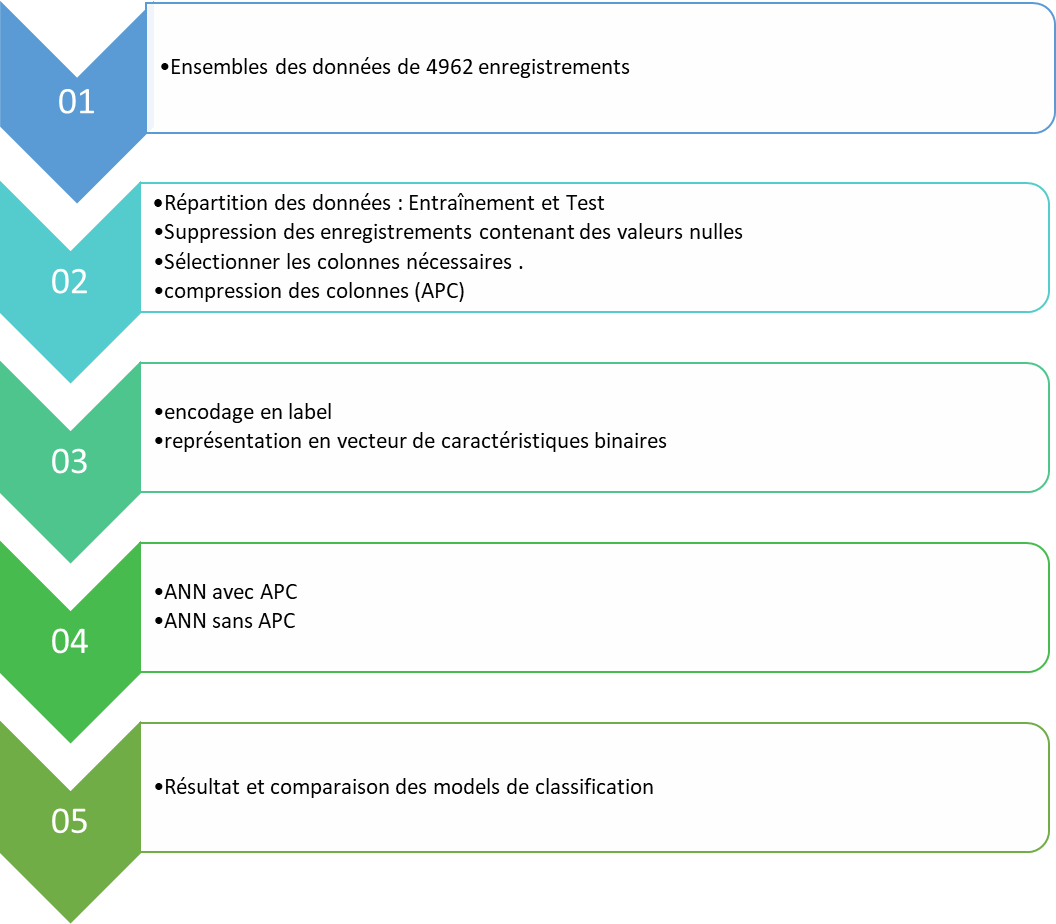
\includegraphics[scale=0.45]{Images/Chapter4/etapes_det.png}
    \caption{Tux, le pingouin}
    \label{fig:18}
\end{figure}

\section{Evaluation des Modèles de Classification}
Dans notre étude, nous avons sélectionné trois mesures de performance essentielles pour évaluer les modèles : la précision, le rappel et l'exactitude (Accuracy en anglais). Ces mesures ont été choisies pour fournir une évaluation holistique des performances des modèles dans la classification des données médicales. En plus de ces métriques, nous avons également pris en compte le score F1
\begin{table}[htbp]
    \centering
    \begin{tabular}{l|l|c|c|c}
        \multicolumn{2}{c}{}&\multicolumn{2}{c}{prédite}&\\
        \cline{3-4}
        \multicolumn{2}{c|}{}&Positive&Negative&\multicolumn{1}{c}{Total}\\
        \cline{2-4}
        \multirow{2}{*}{réelle }& Positive & $VP$ & $FP$ & $VP+FP$\\
        \cline{2-4}
        & Negative & $FN$ & $VN$ & $FN+VN$\\
        \cline{2-4}
        \multicolumn{1}{c}{} & \multicolumn{1}{c}{Total} & \multicolumn{1}{c}{$VP+FN$} & \multicolumn{    1}{c}{$FP+VN$} \\
    \end{tabular}
    \caption{Table caption}
    \label{tab:mytable}
\end{table}

\subsection{Rappel}
Le rappel \textbf{R} est une métrique qui mesure à quelle fréquence un modèle identifie correctement les instances positives (vrais positifs) parmi tous les échantillons positifs réels dans l'ensemble de données.
\[ R = \frac{VP}{VP+FN} \]
\subsection{Précision}
La précision \textbf{P} mesure la proportion d'échantillons correctement identifiés comme positifs parmi tous les échantillons identifiés comme positifs par le modèle. 
\[ P = \frac{VP}{VP+FP} \]

\subsection{Exactitude}
L'exactitude \textbf{E} est une mesure qui évalue la proportion totale d'échantillons correctement classés parmi tous les échantillons dans l'ensemble de données. C'est-à-dire qu'elle mesure la capacité globale du modèle à prédire correctement les classes de tous les échantillons, qu'ils soient positifs ou négatifs.
\[ E = \frac{VP + VN}{VP + VN + FP + FN} \]

\subsection{Score f1}
Le score \textbf{F1} est une métrique de performance qui combine à la fois la précision et le rappel d'un modèle en une seule valeur. Il offre une mesure globale de la capacité du modèle à classer correctement les échantillons positifs tout en minimisant à la fois les faux positifs et les faux négatifs.
\[F1 = \frac{2*Précision*Rappel}{Précision+Rappel} = \frac{2*VP}{2*VP+FP+FN}\]

\subsection{Temps d'entraînemente}
Le temps d'entraînement \textbf{T} du modèle fait référence à la durée nécessaire pour entraîner un modèle d'apprentissage sur un ensemble de données donné . 
\[ \text{T} = t_{\text{fin}} - t_{\text{début}} \]


\section{Optimisation des models de classification}
\subsection{Adam (Estimation de moment adaptatif)}
Ce sont les étapes principales de l'algorithme Adam pour mettre à jour les poids (\ref*{Les poids}) pendant le processus d'entraînement. L'algorithme Adam combine la prise en compte des moments 1 et 2 ainsi que le taux d'apprentissage pour mettre à jour les poids, ce qui lui permet d'améliorer la stabilité et la vitesse du processus d'entrainement dans de nombreux cas. Pour accéder aux poids et aux biais de notre modèle, on peut utiliser les fonctions \textbf{model.weights} et \textbf{model.bias.numpy()}.
\begin{enumerate}
    \item \textbf{Initialisation }:Les poids du modèle sont initialisés de manière aléatoire.
    \item \textbf{Calcul des Gradients }:Les gradients des poids du modèle par rapport à la fonction de coût sont calculés à l'aide de la technique de la rétropropagation du gradient.
    \item \textbf{Mise à jour des moments 1 et 2 }:Les moments 1 et 2 sont mis à jour en utilisant les formules suivantes :
    \[ m_t = \beta_1 \cdot m_{t-1} + (1 - \beta_1) \cdot \text{gradient}_t \]
    \[ V_t = \beta_2 \cdot V_{t-1} + (1 - \beta_2) \cdot \text{gradient}_{t}^{2} \]
    (\(t\) est le temps actuel et \(\beta_1\) et \(\beta_2\) sont des paramètres qui contrôlent l'importance des moments.)
    \item \textbf{Correction des biais 1 et 2 }:Les biais 1 et 2 sont corrigés pour compenser les biais initiaux :
   \[ m_{t_{\text{corr}}} = m_t (1 - \beta_1^t)\]
   \[V_{t_{\text{corr}}} = V_t (1 - \beta_2^t)\]
    \item \textbf{Mise à jour des poids }:Les poids sont mis à jour en utilisant la formule suivante :
    \[W_{t+1} = W_t - \left(lr \cdot \left(\sqrt{v_{t_{\text{corr}}} + \epsilon} \right) \cdot m_{t_{\text{corr}}} \right)\]
\[(lr \text{ est le taux d'apprentissage et } \epsilon \text{ est une petite valeur pour éviter la division par zéro.})\]
    \item \textbf{Répétition }:Les étapes 2 à 5 sont répétées jusqu'à ce qu'une condition d'arrêt spécifiée soit remplie.
\end{enumerate}

\subsection{SGD (Descente de gradient stochastique) }
Ce sont les principales étapes de l'algorithme SGD pour mettre à jour les poids pendant le processus d'entraînement. Les poids sont mis à jour en fonction du gradient calculé et du taux d'apprentissage. Les étapes sont appliquées à chaque échantillon ou lot de données dans le cas de l'entraînement par mini-lots (mini-batch training) ou à chaque donnée dans le cas de l'entraînement par lots complets (batch training). Le processus est répété jusqu'à ce que les conditions spécifiées, telles que le nombre de cycles ou l'atteinte de la précision souhaitée, soient remplies
\begin{enumerate}
    \item \textbf{Initialisation }:Les poids du modèle sont initialisés de manière aléatoire.
    \item \textbf{Calcul des gradients }:Les gradients des poids du modèle par rapport à la fonction de coût sont calculés en utilisant la technique de la rétro propagation du gradient.
    \item \textbf{Mise à Jour des poids }:Les poids sont mis à jour en utilisant la formule suivante :
    \[W_{t+1} = W_t - lr \cdot \text{gradient}(t)\]
    (où \( W_t \) représente les poids actuels, \( W_{t+1} \) est le poids mis à jour, et \( lr \) est le taux d'apprentissage.)
    \item \textbf{Répétition }:Les étapes 2 et 3 (calcul des gradiant + mise à jour de poids) sont répétées pour chaque donnée d'entraînement ou pour un nombre spécifié de cycles (epochs) jusqu'à ce qu'un critère d'arrêt spécifié soit atteint
\end{enumerate}

\section{Pertes des modèle de classification }
Dans les modèles de classification, l'optimiseur utilise les informations de la fonction de perte pour ajuster les poids du modèle. Son objectif est de réduire l'erreur de prédiction au fil du temps. En somme, la fonction de perte fournit une mesure de performance que l'optimiseur utilise pour guider le processus d'optimisation vers la solution optimale.
\subsection{Entropie croisée catégorielle eparses}
La fonction de perte "entropie croisée catégorielle éparses", est couramment utilisée dans les problèmes de classification où les étiquettes sont fournies sous forme d'entiers plutôt que sous forme de vecteurs multi-étiquette. Elle mesure la différence entre les prédictions du modèle et les étiquettes réelles associées aux données. La formule mathématique de la fonction de perte entropie croisée catégorielle éparses est la suivante :
\[
\text{SCE}(y,t) = -\sum_i t_i \cdot \log(y_i)
\]
\begin{itemize}
    \item $\text{SCE}$ représente l'entropie croisée catégorielle éparses.
    \item $y$ est la sortie (prédiction) produite par le modèle.
    \item $t$ est la valeur réelle cible (étiquette), où $t_i$ est soit 0 soit 1.
    \item $\log$ représente le logarithme naturel.
    \item La somme est effectuée sur toutes les classes $i$.
\end{itemize}
Cette fonction de perte mesure la dissimilarité entre la distribution de probabilité prédite par le modèle ($y$) et la distribution de probabilité réelle ($t$) pour chaque exemple dans l'ensemble de données. Elle est souvent utilisée dans les tâches de classification avec plusieurs classes.
\newpage\section{Conclusion}
Dans ce chapitre, nous avons clarifié la stratégie générale de notre travail en exposant clairement nos objectifs. Nous avons décrit la méthodologie adoptée pour mener une étude comparative entre deux modèles de classification des symptômes, combinés à différentes méthodes d’optimisation été adopté. Nous avons expliqué que la mise en œuvre de cette comparaison sur un corpus de données réelles sera détaillée dans le prochain chapitre, où nous présenterons également les résultats obtenus, ainsi que leur analyse approfondie et leur discussion.
















% \section{Les références}

% Les listes de références sont gérées en \LaTeX\ à l'aide de l'outil Bib\TeX\, logiciel de gestion de références bibliographiques développé principalement à cet effet. Voici le lien suivant qui explique en détail comment utiliser Bib\TeX\ :  \url{https://fr.overleaf.com/learn/latex/Bibliography_management_with_bibtex}

% Veuillez suivre le style de référence IEEE, pour cela, vous pouvez choisir, par exemple, le style de référence \verb|IEEEtranN|, ce dernier qui nécessite l'invocation du package \verb|natbib| en ajoutant \verb+\usepackage[numbers]{natbib}+ au préambule.

% \cite{4}, \cite{2}, \cite{3}, \cite{5}, \cite{1}, ...


% \section{...}
% \noindent
% Acronym of "Intelligence Artificielle": \acrshort{ia} \\
% Meaning of MI: \acrlong{mi}
